\chapter{System Design}
In this chapter we will discuss the architecture and design of the \textbf{TechBook} system. In the following sections we will present code snippets and visual diagrams to help portray a basic understanding of the application design. The architecture is modeled on what is known as the MEAN stack and which resembles a three tier architecture. MEAN is a free open-source software stack for building dynamic websites and supports the MVC (Model View Controller) architecture. The contents of this chapter will be seperated into the Data Tier, Logic Tier and Presentation Tier.




\begin{figure}[H]
\begin{minipage}{.5\textwidth}  %listing bloc will have 50% of the line width 
\lstset{linewidth = 4cm, breaklines=true} %set your listing lines widths, and set breaklines to true
\begin{itemize}
\item Database \textbf{MongoDB}
\item Server \textbf{Node.js/express}
\item Client \textbf{Angular.js}
\end{itemize}

\end{minipage}
\qquad %space between listing bloc and the figure
\begin{minipage}{0.4\textwidth} %figure will have the remaning 40% of the line width
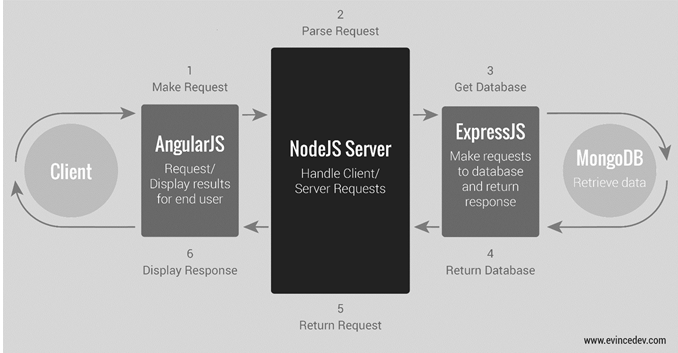
\includegraphics[scale=.4]{img/mvc.png} %the image must be resized or scaled if needed
\caption{MEAN Stack}
\end{minipage}
\end{figure}

% ========================== Databases ========================== 
\section{Database}
For the database adapting the MEAN architecture we used MongoDB.

\subsection{Mongoose}
Harnessing the true power of the Mean stack we used the mongoose object modelling package for Node. Mongoose enabled us to have access to the full suite of MongoDB commands to perform CRUD (Create, Read, Update, Delete) operations. 


To use mongoose we used the following command in the project directory to add it to our Node project:
\begin{lstlisting}[language=DOS]
npm install mongoose --save
\end{lstlisting}

Once the package was installed we have to access it in our project :
\begin{lstlisting}[language=JavaScript]
var mongoose = require('mongoose');
\end{lstlisting}

Finally to connect to our MongoDB:
\begin{lstlisting}[language=JavaScript]
// Connect to the mongodb using settings from the config file
mongoose.connect(config.database, { promiseLibrary: require('bluebird') })
  .then(() =>  console.log('\x1b[32m%s\x1b[0m', 'INFO: Connection to database succesfull'))
  .catch((err) => console.error(err));
\end{lstlisting}

\subsection{Mongoose Schema}
Prior to performing CRUD operations we had to define our  mongooses models. These represent documents which can be saved, read and retrieved from our database. The Mongoose Schema is how we define attributes to these documents. To enhance security and the SRP(Single Responsibility Principle) numerous different models were defined and using keys enabled the ability to map relationships to other models.

\begin{figure}[H]
  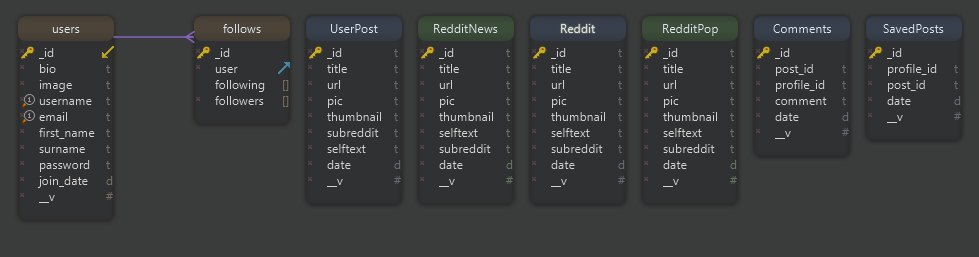
\includegraphics[width=\linewidth]{img/schemas.PNG}
  \caption{MongoDB models}
  \label{fig:schema}
\end{figure}

Figure ~\ref{fig:userscema} below shows how the UserSchema was defined in user.js. The schema was designed to add maximum functionality while also protecting the system from having invalid objects added to the database. There are a few things to note about this particular schema.
\begin{itemize}
\item \textbf{Uniqueness} : The \textit{username} and \textit{email} fields are set to unique. This ensures a user can only have one account per email and that the username will not not cause issues when a search query is performed.
\item \textbf{Required} : The \textit{username}, \textit{firstname},\textit{surname} and \textit{password} fields are required. These represent the bare minimum that must be initialised to have a valid account.
\item \textbf{Default} : The \textit{joindate},\textit{bio} and \textit{image} are set to default. This allows a faster user registration with a default image used, the join date set to the current date and a generic bio that can all be updated using the settings link.
\end{itemize}

\begin{lstlisting}[language=JavaScript,caption={Defining User Schema},captionpos=b,label={fig:userscema}]
// Schema used to 'filter' data to be stored in the 'UserSchema' collection in mongo
var UserSchema = new mongoose.Schema({
  username: {
    type: String,
    unique: true,
    required: true
  },
  email: {
    type: String,
    unique: true,
  },
  first_name: {
    type: String,
    required: true
  },
  surname: {
    type: String,
    required: true
  },
  join_date: {
    type: Date,
    default: Date.now
  },
  bio: {
    type: String,
    default: 'Tell me about yourself'
  },
  image:{
    type: String,
    default: 'profile.jpg'
  },
  password: {
    type: String,
    required: true
  }
});

\end{lstlisting}

\subsection{Password hashing}
To ensure the highest standard of security any confidential user information should never directly be stored in a database. Mongoose allows us to define functions using 'pre(function,functionToExecute)' that executes prior to saving a document. Bcrypt a node-module that simplifies hashing can be used to both encrypt and decrypt sensitive data. Combining the use of these technologies when a user account is created or modified, the password is hashed before saving the document and in turn the hashed value of the password is saved in the database thus protecting the origonal password being exposed in the event of a malicious attack.

\begin{lstlisting}[language=JavaScript,caption={Password Hashing},captionpos=b,label={fig:presave}]
// define pre hook for document
UserSchema.pre('save', function (next) {
  var user = this;
  // if password new or edited
  if (this.isModified('password') || this.isNew) {
    // generate a salt and process data for 10 rounds
    bcrypt.genSalt(10, function (err, salt) {
      if (err) {
        return next(err);
      }
      // generate a hash of password
      bcrypt.hash(user.password, salt, null, function (err, hash) {
        if (err) {
          return next(err);
        }
        user.password = hash;
        next();
      });
    });
  } else {
    return next();
  }
});

\end{lstlisting}
Ensuring the password is hashed is of major importance but equally as crucial is the ability to be able to compare the hashed value with a password entered by a user attempting to log in. To achieve this we were able to attach a comparePassword function to the UserSchema which executes the compare method from the bcrypt module and checks for a match between the password entered and the hashed password stored in the database as shown in Figure ~\ref{fig:passcheck}. 
\begin{lstlisting}[language=JavaScript,caption={Password Comparision},captionpos=b,label={fig:passcheck}]
// compare password for log in
UserSchema.methods.comparePassword = function (passw, cb) {
  bcrypt.compare(passw, this.password, function (err, isMatch) {
    if (err) {
      return cb(err);
    }
    cb(null, isMatch);
  });
};
\end{lstlisting}

\subsection{JSON Web tokens}
% ========================== Authentication ========================== 
\section{Authentication}
What database like

% ========================== API Calls ========================== 
\section{API/HTTP}
How we designed api calls/
insert info from swagger

% ========================== UI ========================== 
\section{Client UI}
The presentation tier is based on the Angular front-end web framework. In contrast to traditional multiple page web applications the Client is presented as a single page application in which components are injected into. In this section we will look at the Angular app structure, the services which allow us to interact with our node js server and the finished view of the pages.

\subsection{Angular folder structure}

\subsection{Angular Services}
The Angular services allow our application to interact and access data from our database via the node server. Thus keeping data retrieval separate to page functions. In the services we provide the logic to process HTTP requests to the API to perform CRUD operations on the data served by the Node.js/ExpressJS server. 

\subsection{Page views}

How we designed the ui
few screenshots off finished site


\begin{itemize}
\item Architecture, UML etc. An overview of the different components of the system. Diagrams etc… Screen shots etc.
\end{itemize}

\begin{table}[h]
  \centering
  \begin{tabular}{x{2cm}p{3cm}}
    \toprule \\
    Column 1 & Column 2 \\
    \midrule \\
    Rows 2.1 & Row 2.2 \\
    \bottomrule
  \end{tabular}
  \caption{A table.}
  \label{table:mytable}
\end{table}